%% Homology-leakage audit -- OUP Bioinformatics Advances (Modern, Large), author-year.
%% Every numeric slot is filled from results/PAPER_NUMBERS.md (frozen); see the
%% per-line %% [slot] comments and the hand-back for the full slot list.
\documentclass[webpdf,modern,large,namedate]{oup-authoring-template}%
%% modern,large = "Modern Large"; namedate = author-year (natbib authoryear).
%% numbered sections are the class default (we omit `unnumsec`).

\graphicspath{{Fig/}}
\emergencystretch=3em % absorb overfull lines from long underscore dataset names / the repo URL in the two-column layout

\begin{document}

\journaltitle{Bioinformatics Advances}
\DOI{DOI added during production}% TODO: pre-acceptance stub -- DOI assigned by OUP at production
\copyrightyear{2026}% TODO: confirm copyright year at acceptance
\pubyear{2026}% TODO: confirm publication year at acceptance; Volume/Issue stay blank until production (running header shows them empty -- no \volume/\issue command yet)
\access{Advance Access Publication Date: Day Month Year}% TODO: pre-acceptance stub -- publication date set at production
\appnotes{Original Paper}

\firstpage{1}% TODO: pre-acceptance stub -- first page assigned at production

%\subtitle{Genome analysis}

\title[Homology leakage changes which model wins]{Homology leakage selectively changes which model wins on genomic sequence-classification benchmarks}

%% ===== Author / affiliation =====
\author[1,$\ast$]{Rikhin Kavuru}
\address[1]{\orgname{Independent Researcher}}
\corresp[$\ast$]{Corresponding author. \href{mailto:rikhinkavuru@gmail.com}{rikhinkavuru@gmail.com}}

% TODO: uncomment and fill the received/revised/accepted dates at acceptance
%\received{Date}{0}{Year}
%\revised{Date}{0}{Year}
%\accepted{Date}{0}{Year}

%% NOTE [drop reconciliation]: headline drops are the TEST-SET BOOTSTRAP point
%% estimates with 95% CIs (PAPER_NUMBERS.md S16.2; 1000 resamples, seed 20240524,
%% no refit), all from one internally-consistent run so each point lies inside its
%% CI: ensembl RandomForest k=6 = 16.4 pts (0.164, CI [0.158,0.170]); nontata =
%% 10.8 pts (0.108, CI [0.099,0.118]). The 3-seed frozen tables (S3/S5) give
%% 15.6/12.1 pts and the 5-seed-mean corrected accuracies (S16.1) give 16.0/12.2;
%% these differ by RandomForest thread-nondeterminism (~0.004) and the seed-0 vs
%% mean corrected split, and are all documented in PAPER_NUMBERS S16. CIs establish
%% significance (both leaky drops exclude zero; all clean deltas include zero).
\abstract{
\textbf{Motivation:} Benchmarks for DNA sequence classification underpin method comparison, but standard train/test splits rarely control for sequence homology. When near-identical sequences span the split, models can score well by memorizing near-duplicates rather than generalizing, and the consequences for method comparison have not been systematically characterized.\\
\textbf{Results:} We audit seven binary datasets from the Genomic Benchmarks suite, quantifying train/test homology by exact $k$-mer Jaccard similarity and re-evaluating four classifiers under a homology-aware re-split that confines near-duplicate clusters to one side. Two datasets are materially leaky (38--41\% of test sequences have a training near-duplicate); correcting the split removes 16.4 and 10.8 points of random-forest accuracy on these two (95\% bootstrap CIs $[15.8, 17.0]$ and $[9.9, 11.8]$), while the remaining five show no significant change (all clean-dataset accuracy deltas have 95\% bootstrap confidence intervals including zero). Crucially, leakage does not merely inflate scores---it changes which method appears best: the apparent best model on the standard split---a random forest---is demoted after correction, to third of four on the nonTATA-promoter dataset and to last on the Ensembl-enhancer dataset, whereas rankings on all five clean datasets are preserved. A homology-graded analysis indicates the mechanism is largely memorization of label-carrying near-duplicates: cleanly on the Ensembl-enhancer dataset, and only partially on the nonTATA-promoter dataset, where the random forest retains a genuine advantage on truly novel sequences. We provide a per-dataset leakage report card and a drop-in homology-aware splitter.\\
\textbf{Availability and implementation:} Code and data are available at \url{https://github.com/rikhinkavuru/homology-leakage-genomic-benchmarks}; the audit is CPU-only and fully reproducible.}

\keywords{data leakage, sequence homology, benchmark evaluation, genomics, model ranking}

\maketitle

\section{Introduction}

Machine learning for DNA sequence classification is now routine, and benchmark suites have become the default proving grounds for new methods. The Genomic Benchmarks collection \citep{gresova2023} is widely used precisely because it is small, accessible, and quick to run, making it a natural first stop when comparing models. The scientific value of any such suite, however, rests entirely on one assumption: that its train/test split measures generalization rather than recall of the training data.

Sequence homology threatens this assumption. We use \emph{homology leakage} to mean the situation in which sequences related by shared ancestry or near-duplication appear on both sides of a split. A model can then succeed on the test set by recognizing memorized near-copies of training examples rather than by learning generalizable signal, so reported accuracy overstates true generalization. This failure mode is increasingly documented across biological machine learning, from regulatory-genomics regression to protein-interaction prediction and virtual screening (Section~\ref{sec:related}).

What remains underexamined is the structure and the consequences of this leakage within a single, widely used suite. Prior work documents inflated scores within individual leaky domains, but three questions are open: (i) whether leakage is uniform across a suite or concentrated in specific datasets; (ii) whether it changes \emph{which} method appears best, not merely the absolute scores; and (iii) whether a controlled, within-study contrast against clean datasets can isolate leakage as the cause rather than a confound.

We address these questions for the Genomic Benchmarks binary classification suite. Our contributions are:
\begin{itemize}
\item a homology audit of the binary suite with a matched clean-versus-leaky control, showing that leakage is dataset-specific rather than universal;
\item evidence that leakage \emph{selectively changes which model appears best} on leaky datasets while leaving rankings on clean datasets intact;
\item a homology-graded analysis indicating the mechanism is memorization of label-carrying near-duplicates, demonstrated cleanly on one dataset and partially on another; and
\item a practical per-dataset report card and an open, drop-in homology-aware splitter.
\end{itemize}
The entire study is CPU-only, deterministic, and reproducible, with all seeds logged and no external services required.

\section{Related work}\label{sec:related}

Homology leakage is increasingly recognized as a benchmarking hazard. hashFrag \citep{rafi2025} shows that homologous sequences spanning genomic train/test splits inflate the apparent performance of neural models and, in particular, that test performance scales with similarity to the training set; it provides tools to detect and partition such data. In protein--protein interaction prediction, \citet{bushuiev2024} show that sequence- and metadata-based splits leave most test cases with near-duplicate counterparts, producing benchmarks that reward overfitting capacity rather than generalization. PINDER \citep{kovtun2024} similarly demonstrates that de-leaked test sets sharply reduce reported performance, including for AlphaFold-Multimer. In virtual screening, an audit of LIT-PCBA \citep{huang2025} shows that a trivial memorization baseline can match sophisticated methods once leakage is accounted for.

We differ from these studies in three ways. Each prior study examines a single leaky domain without a matched clean control; we audit a whole suite and find that leakage is dataset-specific, using a within-study leaky-versus-clean contrast to isolate it as the cause. Where prior work documents inflated absolute scores, we show that leakage changes which model appears best, quantified against clean datasets on which rankings are preserved. And we target the Genomic Benchmarks classification suite specifically---the community's default quick-evaluation benchmark---for which no such audit exists. Methodologically, we adapt the similarity-graded analysis used by hashFrag for regression to the classification setting and extend it to the consequence for method ranking.

\section{Methods}

\subsection{Datasets}
We study the seven binary datasets of the Genomic Benchmarks suite \citep{gresova2023}, and additionally report the three-class \textit{human\_ensembl\_regulatory} set separately. Per-dataset sizes, sequence lengths, and class balance are given in Table~\ref{tab:datasets}. Sizes range from 6{,}914 (\textit{drosophila\_enhancers\_stark}) to 174{,}756 (\textit{human\_ocr\_ensembl}) sequences; sequence lengths are fixed within some datasets (e.g.\ 251\,bp for \textit{human\_nontata\_promoters}, 200\,bp for the \texttt{demo\_*} demonstration sets) and variable in others; classes are balanced ($0.50$ positive fraction) except \textit{human\_nontata\_promoters} ($0.544$).

\subsection{Features and models}
Each sequence is represented by overlapping $k$-mer counts for $k\in\{4,6\}$ ($4^k$ features), L2-normalized. We evaluate four classifiers spanning a capacity range: logistic regression (\texttt{C=1.0}, \texttt{max\_iter=5000}), a linear support-vector machine (\texttt{LinearSVC}, \texttt{C=1.0}, \texttt{dual=False}, \texttt{max\_iter=5000}), a random forest (\texttt{150} trees), and gradient-boosted trees (\texttt{HistGradientBoosting}, library defaults). All models use a fixed random seed; we report accuracy in the main text, with AUROC and $F_1$ tabulated in the repository.

\subsection{Homology measurement}
We measure homology by the exact Jaccard similarity of $k$-mer sets with $k=8$, computed for all test--train pairs via sparse binary matrix products (no MinHash approximation). For each test sequence we record its maximum similarity to any training sequence, and define the leakage fraction as the proportion of test sequences whose maximum similarity exceeds a threshold; we report thresholds $0.5$, $0.7$, and $0.9$. We detect near-duplicate leakage via exact $k$-mer Jaccard similarity; this captures near-identical sequences, a detectable and conservative subset of homology leakage in the broader evolutionary sense (diverged homologs with low $k$-mer overlap are not flagged and would, if present, only add undetected leakage).

\subsection{Homology-aware re-split}
To correct leakage we build a similarity graph in which sequences are connected when their $k$-mer Jaccard exceeds $0.7$, take connected components as near-duplicate clusters, and assign whole clusters to either train or test. The assignment preserves the original train/test ratio and class balance and, by construction, guarantees zero residual cross-split similarity above the threshold (verified empirically). We confirm robustness to the clustering threshold (sweeping $0.5/0.7/0.9$) and to removal of the single largest component. Sequence-clustering tools such as CD-HIT \citep{li2006cdhit} and MMseqs2 \citep{steinegger2017mmseqs2} are the established means of homology-aware partitioning in bioinformatics; our exact-Jaccard procedure is a lightweight, dependency-free alternative suited to this audit, and either could substitute in the splitter.

\subsection{Controls}
Three controls isolate and explain the effect. (i) A \emph{random} re-split at matched size and class balance, ignoring clusters, serves as a negative control. (ii) A homology-graded analysis bins test sequences by their maximum similarity to training and reports per-bin accuracy. (iii) A label-concordance analysis records, for each near-duplicate test sequence, whether its nearest training neighbour shares its label.

\subsection{Reproducibility}
All experiments are deterministic with logged seeds, CPU-only, and free of external services. The homology-aware splitter is released as a standalone tool (\texttt{homology\_split.py}, dependencies \texttt{numpy}/\texttt{scipy}). Reported 95\% confidence intervals are percentile bootstrap intervals (the 2.5th and 97.5th percentiles of $1{,}000$ resamples of the per-test-example correctness vector; the resampling unit is the individual test sequence, models are not refit, and the random seed is fixed).

\section{Results}

\subsection{Leakage is dataset-specific}
Of the seven binary datasets, only two---\textit{human\_nontata\_promoters} and \textit{human\_enhancers\_ensembl}---exceed a 10\% near-duplicate test fraction at Jaccard $0.7$ ($0.406$ and $0.384$ respectively); the remaining five are near zero (Table~\ref{tab:reportcard}). The three-class \textit{human\_ensembl\_regulatory} set is likewise clean ($0.005$). Leakage is therefore concentrated, not endemic to the suite.

\subsection{Correcting the split lowers accuracy only on leaky datasets}
%% Drops = test-set bootstrap point + 95% CI (PAPER_NUMBERS S16.2); see NOTE above the abstract.
Under the homology-aware re-split, accuracy drops sharply on the leaky datasets---by $16.4$ points (95\% bootstrap CI $[15.8, 17.0]$) for the random forest on \textit{human\_enhancers\_ensembl} and $10.8$ points (95\% CI $[9.9, 11.8]$) on \textit{human\_nontata\_promoters}---whereas clean-dataset deltas are not statistically significant (all five 95\% bootstrap CIs include zero). Both leaky-dataset random-forest drops are significant (CIs exclude zero). The negative control confirms causation: a random re-split of the same data, at matched size and balance, leaves the leaky-dataset accuracies essentially unchanged (best-model deltas $-0.002$ and $-0.001$ on the enhancer and promoter sets respectively, both 95\% CIs including zero). Only removing homology, not re-splitting per se, lowers the score (Fig.~\ref{fig:controls}).

\subsection{Leakage changes which model appears best}
The consequence for method comparison is the central result. On both leaky datasets the apparent best model on the standard split---a random forest---is demoted after correction, falling from rank~1 to rank~3 on \textit{human\_nontata\_promoters} and from rank~1 to last (rank~4) on \textit{human\_enhancers\_ensembl}, whereas the ranking is preserved on all five clean datasets (Fig.~\ref{fig:ranking}). Summarized by rank correlation, the mean Kendall $\tau$ is $-0.17$ on leaky datasets versus $+0.67$ on clean ones; with only four models $\tau$ is coarse, so we treat it as descriptive support for the concrete demotions above rather than a primary statistic (Fig.~\ref{fig:ranking}). Material rank changes---a best-model demotion by a margin whose accuracy CIs do not overlap---occur on $2/2$ leaky datasets and $0/5$ clean datasets; the clean-dataset changes are swaps between statistically tied models whose 95\% bootstrap CIs overlap, including \textit{drosophila\_enhancers\_stark}'s larger ($\approx0.019$) swap, which is additionally unstable across re-split seeds.

\subsection{The mechanism is memorization of label-carrying near-duplicates}
Binning test sequences by similarity to training reveals the mechanism directly (Fig.~\ref{fig:graded}). On \textit{human\_enhancers\_ensembl}, the random forest scores $1.000$ on near-duplicate test sequences ($\ge0.9$ similarity) but only $0.770$ on novel ones ($<0.5$), a gap of $+0.230$, versus a gap of roughly $0.035$ for the other models; tellingly, on the novel sequences the random forest ($0.770$) is \emph{worse} than the linear SVM ($0.782$). The label-concordance analysis explains why memorization pays: at $\ge0.9$ similarity, $99.95\%$ (nontata) and $99.99\%$ (ensembl) of near-duplicate test sequences share the label of their nearest training neighbour, so a model that recognizes a near-copy is correct essentially for free. On \textit{human\_enhancers\_ensembl} the inflation is confined to the high-capacity model: the random-forest drop is significant (its 95\% CI excludes zero) while the logistic-regression drop is null ($\approx0.000$, 95\% CI $[-0.006, +0.007]$, includes zero), indicating that only the model able to memorize near-duplicates is inflated. Clean datasets have near-empty high-similarity bins, leaving nothing to memorize.

\subsection{Honest scope of the mechanism}
The two leaky datasets differ in how cleanly the memorization account applies. On \textit{human\_enhancers\_ensembl}, two independent evaluation routes agree: the corrected split and a novel-sequences-only ranking both dethrone the random forest. On \textit{human\_nontata\_promoters}, these routes diverge ($\tau=-0.67$ between the corrected and novel-only rankings): the random forest is demoted under the corrected split but remains the best model on truly novel sequences (accuracy $0.879$). Its advantage there is therefore partly genuine generalization, not pure test-side memorization. The inflation and ranking-change findings hold for both datasets; the mechanistic claim is clean for \textit{human\_enhancers\_ensembl} and partial for \textit{human\_nontata\_promoters}. This implies a scope limit for homology-aware splitting: it reliably detects and removes near-duplicate leakage, but because cluster removal can also discard legitimately learnable signal, the corrected ranking is not guaranteed to recover the true generalization ranking---as \textit{human\_nontata\_promoters} shows, where the random forest retains a genuine advantage on novel sequences.

\section{Discussion}

Reported performance on some popular genomic benchmarks overstates generalization, and---more consequentially---can mislead about which method is best. Anyone using these suites to rank models risks selecting a method for its capacity to memorize near-duplicates rather than to generalize.

Because the effect is dataset-specific, the contribution is constructive rather than purely cautionary: not ``these benchmarks are broken'' but ``here is which ones to trust, and a tool to certify any new dataset.'' The clean datasets passing the same checks act as a positive control that makes the leaky-dataset findings credible. We package this as a per-dataset report card and a drop-in splitter.

A practical caution concerns scale. Subsampling can mask leakage: \textit{human\_enhancers\_ensembl} appears almost clean at a 20{,}000-sequence subsample (leakage fraction $0.056$ at Jaccard $0.7$) yet is heavily leaky at full scale ($0.384$), because subsampling breaks up near-duplicate pairs. Homology audits must therefore be run at full dataset scale.

Our study has limits. We use classical models rather than deep networks; we expect the mechanism to affect any model prone to memorizing near-duplicates---among the classical models studied, the random forest, the strongest memorizer, is the most inflated---but we do not demonstrate this for deep networks. We use $k$-mer features and exact $k$-mer Jaccard as the similarity proxy (validated against the re-split guarantee), and we examine a single benchmark suite. Natural extensions are deep models, additional suites, and alignment-based similarity measures.

%% ===================== TABLES =====================

%% [Methods 3.1 / PAPER_NUMBERS.md S1 descriptors (+S13 report card for the 3-class n)]
\begin{table*}[tbp]
\begin{center}
\begin{minipage}{\textwidth}
\caption{Datasets in the Genomic Benchmarks binary suite (and the optional three-class set). Lengths are the median (with min--max range where variable); class balance is the positive-class fraction (binary).\label{tab:datasets}}
\footnotesize\setlength{\tabcolsep}{5pt}\begin{tabular}{@{}lrlll@{}}
\toprule
Dataset & $n$ (full) & Length (bp) & Class balance & Test fraction\\
\midrule
human\_nontata\_promoters          & 36{,}131  & 251              & 0.544 & 0.25\\
human\_enhancers\_ensembl          & 154{,}842 & 269 (2--573)     & 0.500 & 0.20\\
human\_ocr\_ensembl                & 174{,}756 & 315 (71--593)    & 0.500 & 0.20\\
human\_enhancers\_cohn             & 27{,}791  & 500              & 0.500 & 0.25\\
demo\_coding\_vs\_intergenomic\_seqs & 100{,}000 & 200              & 0.500 & 0.25\\
demo\_human\_or\_worm               & 100{,}000 & 200              & 0.500 & 0.25\\
drosophila\_enhancers\_stark       & 6{,}914   & 2142 (236--3237) & 0.500 & 0.25\\
\midrule
human\_ensembl\_regulatory (3-class) & 289{,}061 & 401 (89--802)  & 3 classes & 0.20\\
\botrule
\end{tabular}
\end{minipage}
\end{center}
\end{table*}

%% [Results 4.1 / PAPER_NUMBERS.md S13 leakage report card]
\begin{table*}[tbp]
\begin{center}
\begin{minipage}{\textwidth}
\caption{Leakage report card. Verdict is LEAKY if the full-scale near-duplicate test fraction exceeds $0.1$ at Jaccard $0.7$. ``Acc.\ lost'' is the best-model accuracy change under the homology-aware re-split (original $-$ corrected; positive $=$ accuracy lost under correction); ``Best-model change?'' flags whether the top-ranked model differs after correction, and ``RF rank'' gives the random-forest rank before/after.\label{tab:reportcard}}
\resizebox{\textwidth}{!}{\begin{tabular}{@{}lrrrllrll@{}}
\toprule
Dataset & $n$ (full) & leak@0.7 & leak@0.9 & Verdict & Best model & Acc.\ lost & Best-model change? & RF rank\\
\midrule
human\_nontata\_promoters          & 36{,}131  & 0.406 & 0.225 & \textbf{LEAKY} & RF ($k$=6) & $+0.108$ & yes  & $1\!\to\!3$\\
human\_enhancers\_ensembl          & 154{,}842 & 0.384 & 0.380 & \textbf{LEAKY} & RF ($k$=6) & $+0.164$ & yes  & $1\!\to\!4$\\
demo\_coding\_vs\_intergenomic\_seqs & 100{,}000 & 0.078 & 0.024 & clean & LR ($k$=6) & $-0.001$ & no   & $4\!\to\!4$\\
human\_ocr\_ensembl                & 174{,}756 & 0.010 & 0.001 & clean & LR ($k$=6) & $+0.004$ & no   & $4\!\to\!4$\\
demo\_human\_or\_worm               & 100{,}000 & 0.012 & 0.003 & clean & LR ($k$=6) & $-0.004$ & no   & $4\!\to\!4$\\
drosophila\_enhancers\_stark       & 6{,}914   & 0.016 & 0.006 & clean & LR ($k$=6) & $+0.012$ & no   & $2\!\to\!3$\\
human\_enhancers\_cohn             & 27{,}791  & 0.001 & 0.000 & clean & LR ($k$=6) & $-0.004$ & no   & $4\!\to\!4$\\
\midrule
human\_ensembl\_regulatory (3-class) & 289{,}061 & 0.005 & 0.001 & clean & RF ($k$=4) & $-0.010$ & n/a & n/a\\
\botrule
\end{tabular}}
\end{minipage}
\end{center}
\end{table*}

%% ===================== FIGURES =====================

\begin{figure}[tbp]
\centering
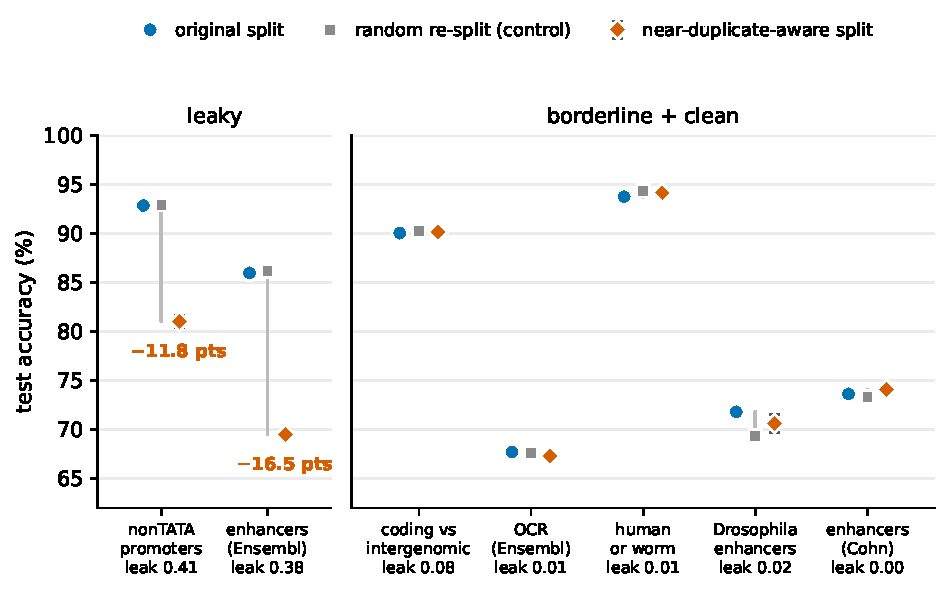
\includegraphics[width=\linewidth]{fig_controls}
\caption{Original split versus random re-split (negative control) versus homology-aware re-split, best model per dataset. Only the homology-aware split lowers accuracy, and only on leaky datasets. The $y$-axis is truncated at 50\% (not 0\%) to make the homology-aware accuracy drop visible; bars span best-model accuracies of roughly 70--93\%.}\label{fig:controls}
\end{figure}

\begin{figure*}[tbp]
\centering
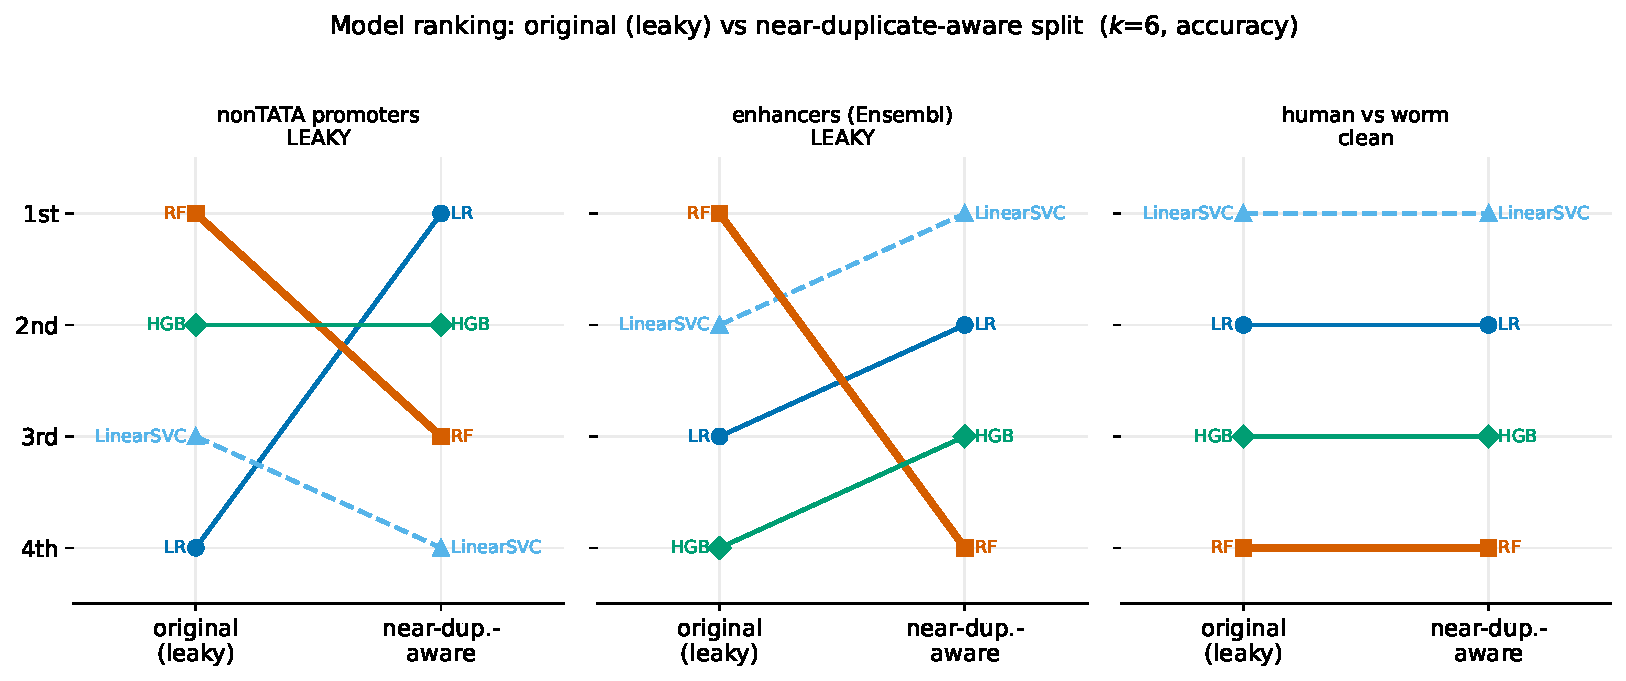
\includegraphics[width=\textwidth]{fig_ranking_inversion}
\caption{Model rankings on the original (leaky) split versus the homology-aware split ($k$=6, accuracy). The random forest is dethroned on the leaky datasets (left, middle) but rankings are stable on a clean control (right). Per-panel $\tau$ is the rank correlation for that dataset; on enhancers (Ensembl) the random forest's move to last flips only its own pairs, giving $\tau\approx0$, while the $-0.17$ in \S4.3 is the mean across both leaky datasets.}\label{fig:ranking}
\end{figure*}

\begin{figure*}[tbp]
\centering
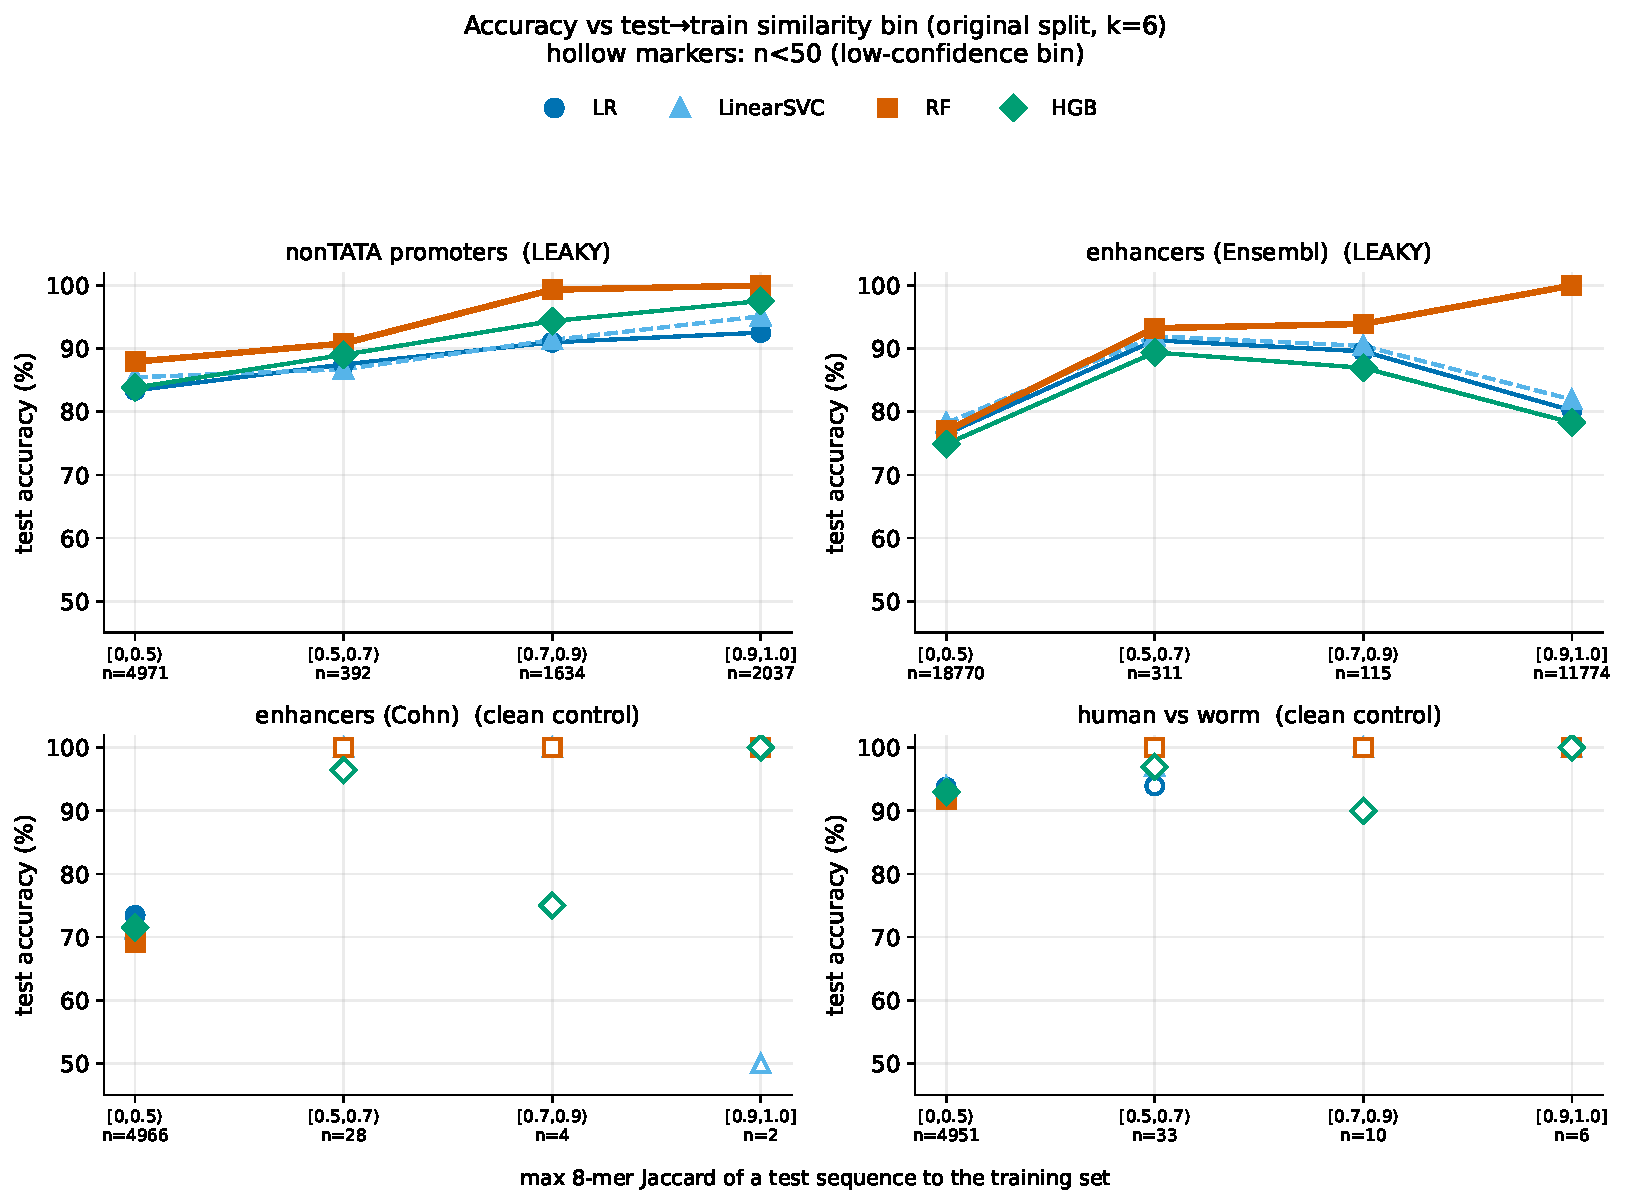
\includegraphics[width=\textwidth]{fig_graded_performance}
\caption{Accuracy as a function of the test-to-train similarity bin (original split, $k$=6). On leaky datasets the random forest is near-perfect on high-similarity (near-duplicate) test sequences and falls on dissimilar ones; clean controls have near-empty high-similarity bins (hollow markers: $n<50$).}\label{fig:graded}
\end{figure*}

\section*{Funding}
This research received no specific grant from any funding agency in the public, commercial, or not-for-profit sectors.

\section*{Conflict of Interest}
None declared.

\section*{Data Availability}
All code required to reproduce the analyses, along with the leakage report card, figures, and the homology-aware splitter tool, is available at \url{https://github.com/rikhinkavuru/homology-leakage-genomic-benchmarks}. The Genomic Benchmarks datasets analysed here are publicly available and were obtained via the genomic-benchmarks package \citep{gresova2023}; they are not redistributed in our repository.

\bibliographystyle{oup-abbrvnat}
\bibliography{references}

\end{document}
